\section{On Predicting the Future}
\label{sec:predicting_future}

Richard Hamming in \emph{The Art of
Doing Science and Engineering}~\citep{hamming1997art} makes many predictions,
many of which have come to pass. Here are a few examples\footnote{Quotes and
predictions are from chapters 2, 4, and 21 of \citet{hamming1997art}.}
\begin{itemize}
    \item He stated that by ``the year 2020 it would be fairly universal
        practice for the expert in the field of application to do the actual
        program preparation rather than have experts in computers (and ignorant
        of the field of application) do the program preparation.''
    \item He predicted that neural networks ``represent a solution to \emph{the
        programming problem}'', and that ``they will probably play a large part
        in the future of computers.''
    \item He predicted the prevalence of general-purpose rather than
        special-purpose hardware, digital over analog, and high-level
        programming languages all long before the field had decided one way or
        another.
    \item He anticipated the use of fiber-optic cables in place of copper wire
        for communication well before the switch actually took place.
\end{itemize}

These are just a few examples of Hamming's extraordinary prescience. Why was he
so good at predicting the future? Here are a few observations which I think
were key to his ability:

{\bf Practice:} One doesn't get good at predicting the future without actually
practicing at it. Hamming practiced. He reserved every Friday afternoon ``great
thoughts'' in which he mused on the future. But he didn't just predict in
isolation. He made his predictions public, which forced him to put them in a
communicable form and held him accountable. For example, in 1960 Hamming gave a
talk titled ``The History of Computing to the Year 2000'' (you may recognize
the title) in which he predicted how computing would evolve over the several
decades.

{\bf Focus on fundamentals:} In some ways, forecasting the future development
of technology is really just understanding the present state of technology more
than those around you. This requires not just a depth in one field but
non-trivial breadth. This also requires the ability to rapidly assimilate new
knowledge. Mastering the fundamentals builds a strong foundation for both.

{\bf Open mind:} Probably the most important trait Hamming exhibited, and in my
opinion the most difficult to learn, was his ability to keep an open mind.
Keeping an open mind requires constant self-vigilance. Having an open mind one
day does not guarantee having it the next. Having an open mind with respect to
one scientific field does not guarantee having it with respect to another.
Hamming recognized for example that one may be more productive in an office
with the door closed, but he kept his office door open as he believed an ``open
mind leads to the open door, and the open door tends to lead to the open
mind''~\citep[chp. 30]{hamming1997art}.

I'll add to these a few more thoughts. First, the rate of change of progress in
computing and machine learning is increasing. This makes it harder to predict
the distant future today than it was 50 or 100 years ago. These days predicting
the evolution of speech recognition even ten years out strikes me as a
challenge. Hence that's the time frame I'm choosing to work with.

A common saying about technology forecasting is that short-term predictions
tend to be overly optimistic and long-term predictions tend to be overly
pessimistic. This is often attributed to the fact that progress in technology
has been exponential. Figure~\ref{fig:exponential_growth} shows how this
happens if we optimistically extrapolate from the present assuming progress is
linear with time. Progress in speech recognition over the previous decade
(2010-2020) was driven by exponential growth along a few key axes. These
included both compute (e.g. floating-point operations per second) and data set
sizes. Whether or not figure~\ref{fig:exponential_growth} applies to speech
recognition for the coming decade remains to be seen.

\begin{figure}
    \centering
    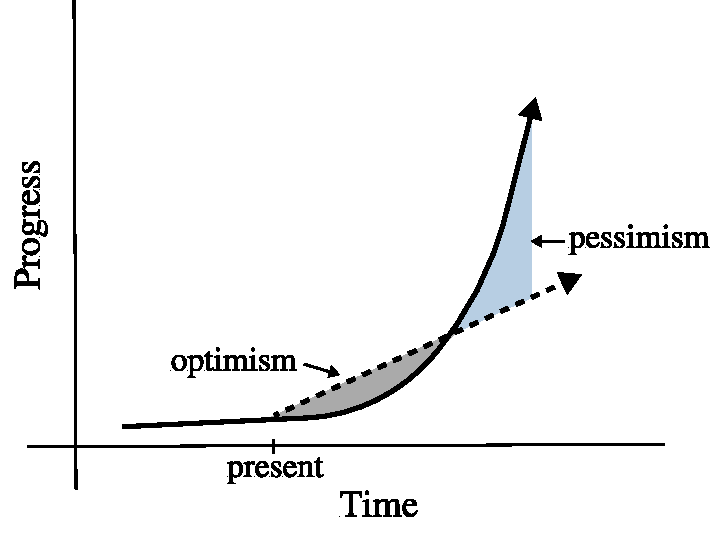
\includegraphics[width=\linewidth]{figures/exponential_growth}
    \caption{The graph depicts progress as a function of time. The linear
    extrapolation from the present (dashed line) initially results in overly
    optimistic predictions.  However, eventually the predictions become
    pessimistic as they are outstripped by the exponential growth (solid
    line).}
    \label{fig:exponential_growth}
\end{figure}

I'm sure a lot of the following predictions will prove wrong. In some ways, the
more controversial predictions I make are really more of an optimistic wishlist
for the future. On that note, let me close this section with the famous words
of the computer scientist Alan Kay\footnote{Alan Kay is best known for
developing the modern graphical user interface and also object-oriented
programming in the Smalltalk programming langauge.}:
\begin{quote}
    \emph{The best way to predict the future is to invent it.}
\end{quote}
